\chapter{Sentry}
Wanneer software ontwikkeld wordt kunnen er natuurlijk verschillende exceptions optreden. Sommige van deze exceptions hebben een kleine impact op de applicatie, maar van andere exceptions wil je vaak dat ze snel worden opgelost.
\newline
De applicaties die ontwikkeld worden maken gebruik van Sentry. Dit is een tool waarbij exceptions die optreden automatisch op een overzichtelijke manier gelogd worden. Zo kunnen we bijvoorbeeld zien hoe vaak een exception optreed.

\section{Container configuratie}
De configuratie van sentry in Docker is anders dat de overige tooling die gebruikt wordt. Daarnaast is het een vereiste dat de Sentry container gekoppeld wordt aan een Postgres database en Redis cache. Dit kan op twee manieren worden gedaan:

\begin{itemize}
	\setlength\itemsep{0em}
	\item Koppelen van Postgres en Redis containers bij het opstarten van Sentry
	\item Environment variabelen meegeven met connectie gegevens voor een externe Postgres en Redis applicatie
\end{itemize}

We hebben ervoor gekozen om binnen docker tevens een Postgres database en Redis cache op te zetten waar Sentry gebruik van maakt. Dit hebben we gedaan aan de hand van de tutorial die te volgens is op \href{https://hub.docker.com/_/sentry/}{de Docker hub pagina van Sentry}.
\newline
\begin{figure}[H]
	\centering
	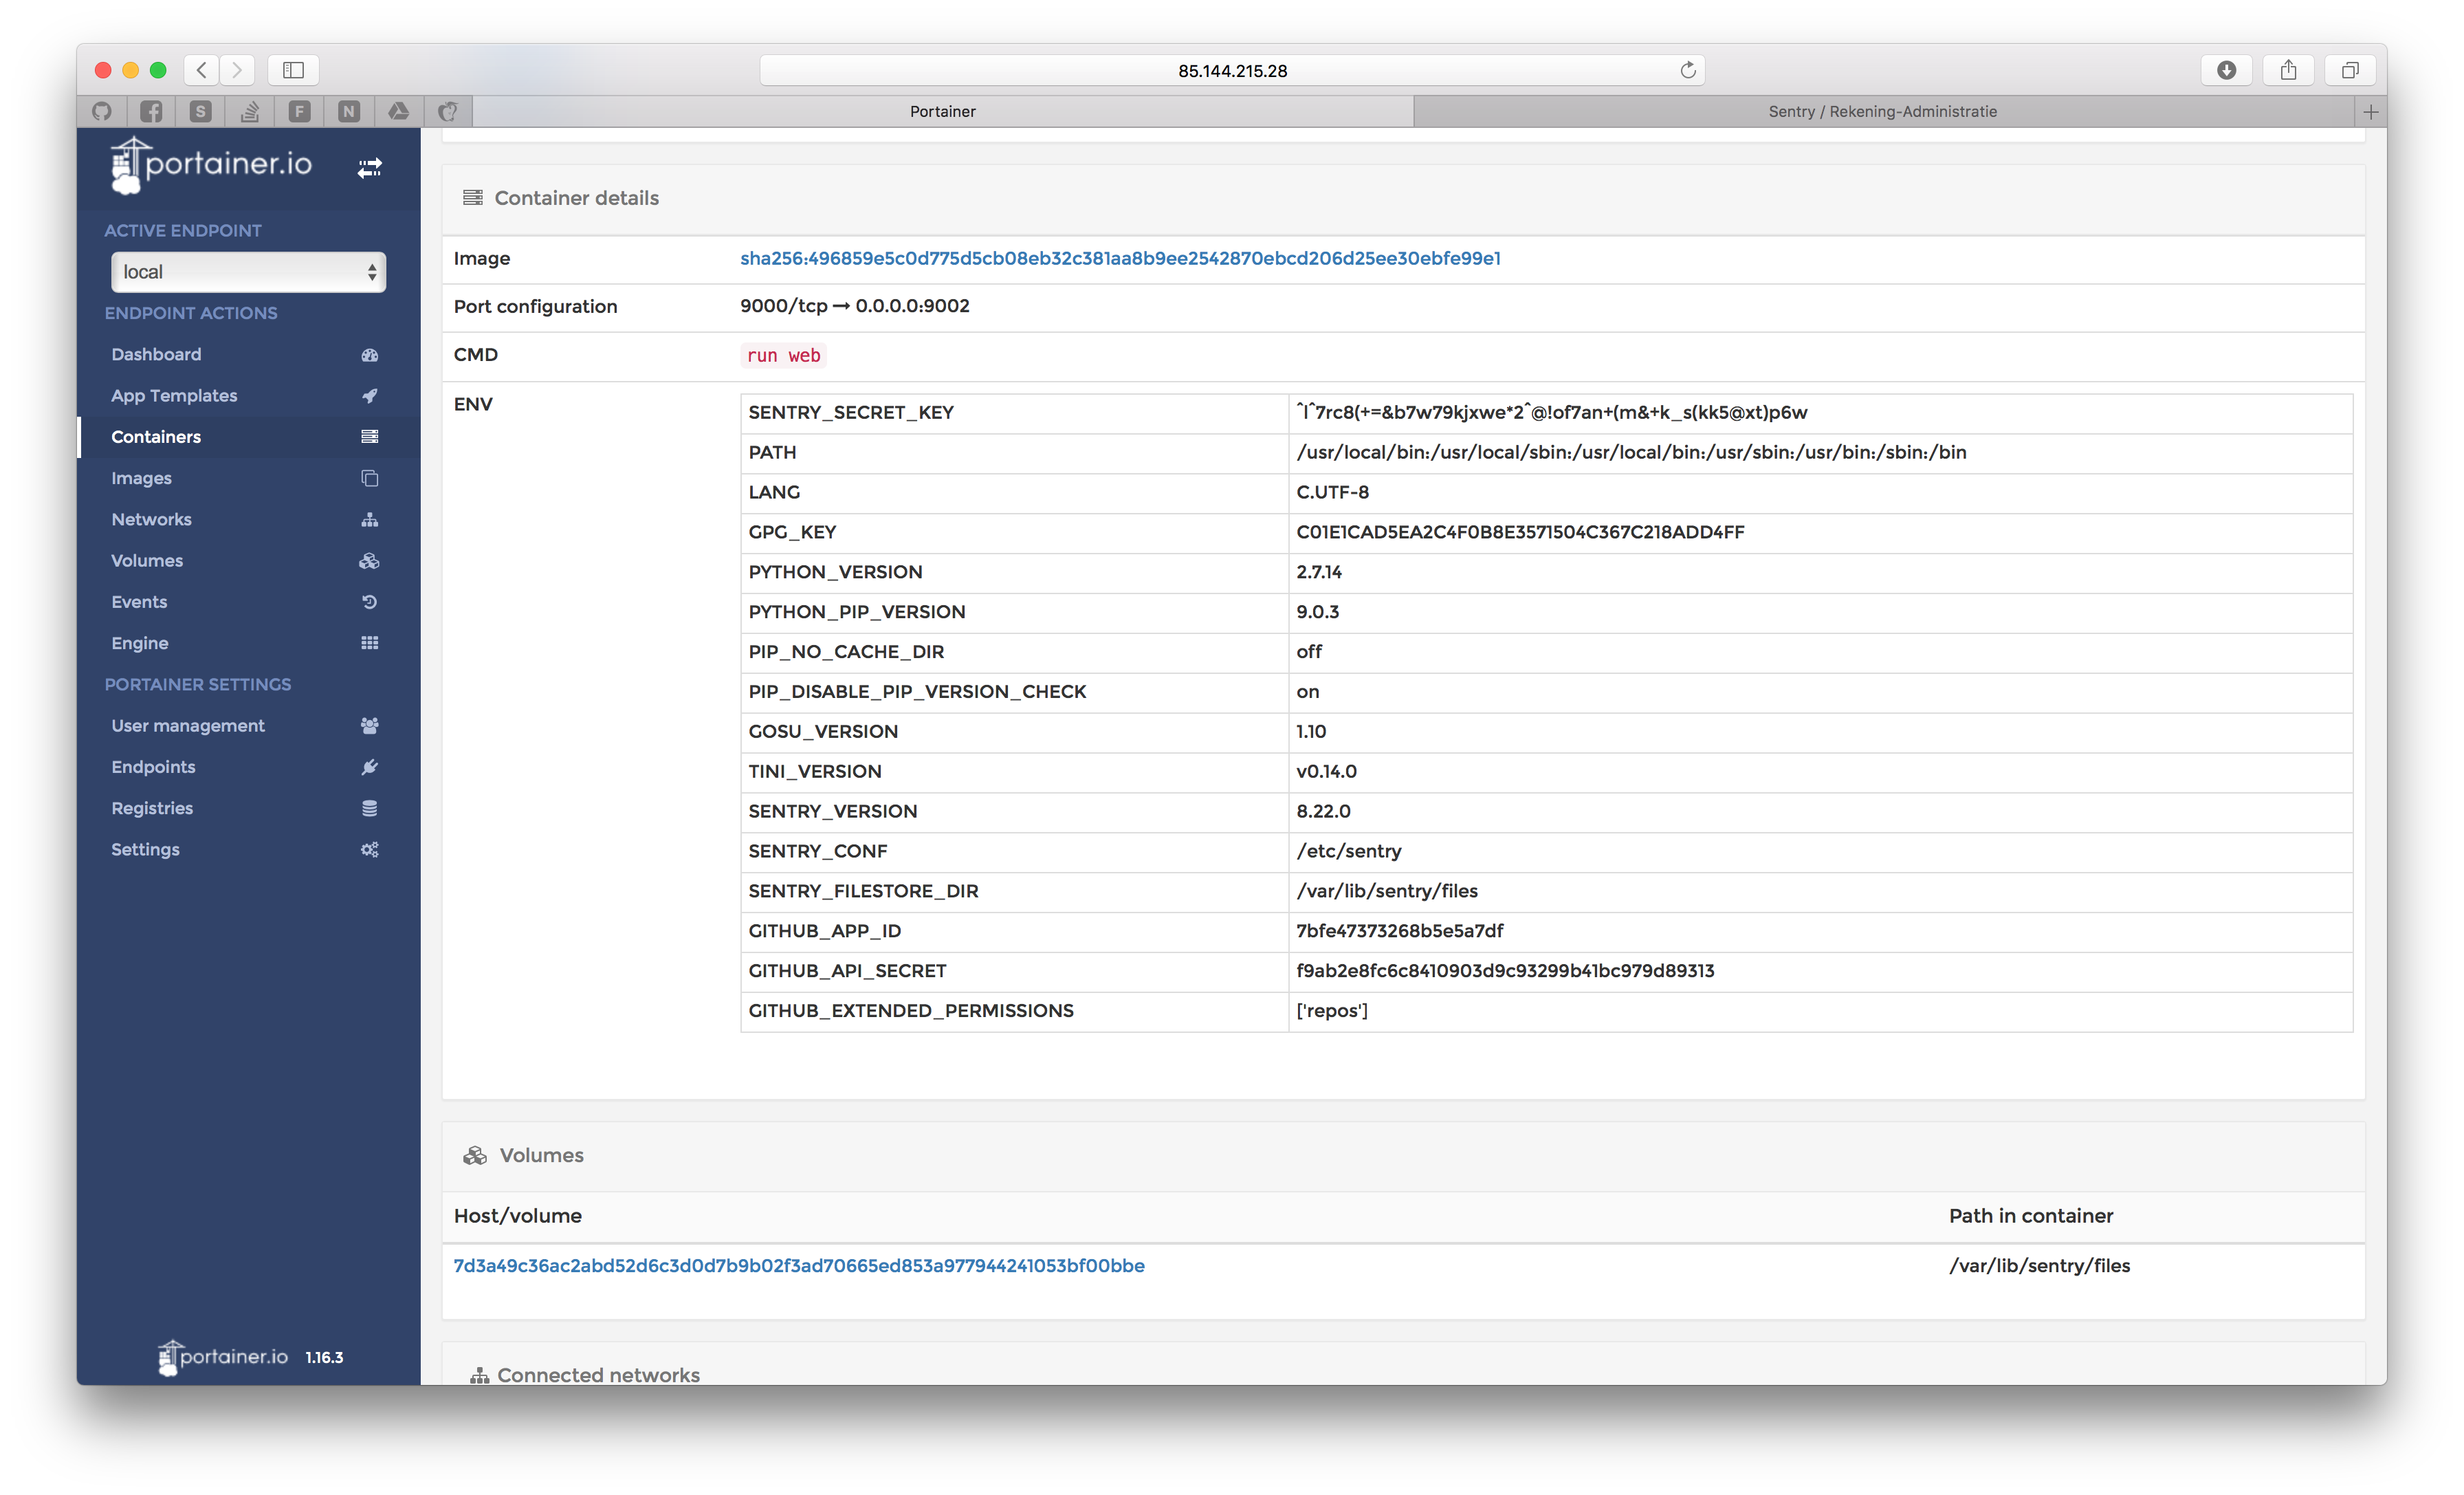
\includegraphics[width=0.95\textwidth]{img/SentryDockerContainer.png}
	\caption{Docker container informatie van Sentry}
	\label{fig:SentryDockerContainer}
\end{figure}

\section{Configuratie van Sentry}
We hebben Sentry geconfigureerd zodat het niet mogelijk is voor iedereen om een nieuw account aan te maken, maar enkel voor de Admin. De reden hiervoor is dat er in exceptions die door Sentry ontvangen is IP's zichtbaar kunnen zijn, en omdat enkel ontwikkelaars van de software toegang mogen hebben tot de exceptions die optreden.
Daarnaast is er voor elke applicatie een project aangemaakt waarin een koppeling met Github is gemaakt. Hierdoor is het mogelijk om van een exception een issue in Github te genereren.
\newline
Om de koppeling met Github te kunnen maken, is binnen Github een nieuwe OAuth applicatie gemaakt. Hierdoor worden een Client ID en Secret ID gegenereerd die door Sentry gebruikt kan worden. Zoals in figuur \ref{fig:SentryDockerContainer} te zien is, worden GITHUB\_APP\_ID, GITHUB\_API\_SECRET en GITHUB\_EXTENDED\_PERMISSIONS meegegeven als environment variabelen voor de Docker container.

\begin{figure}[H]
	\centering
	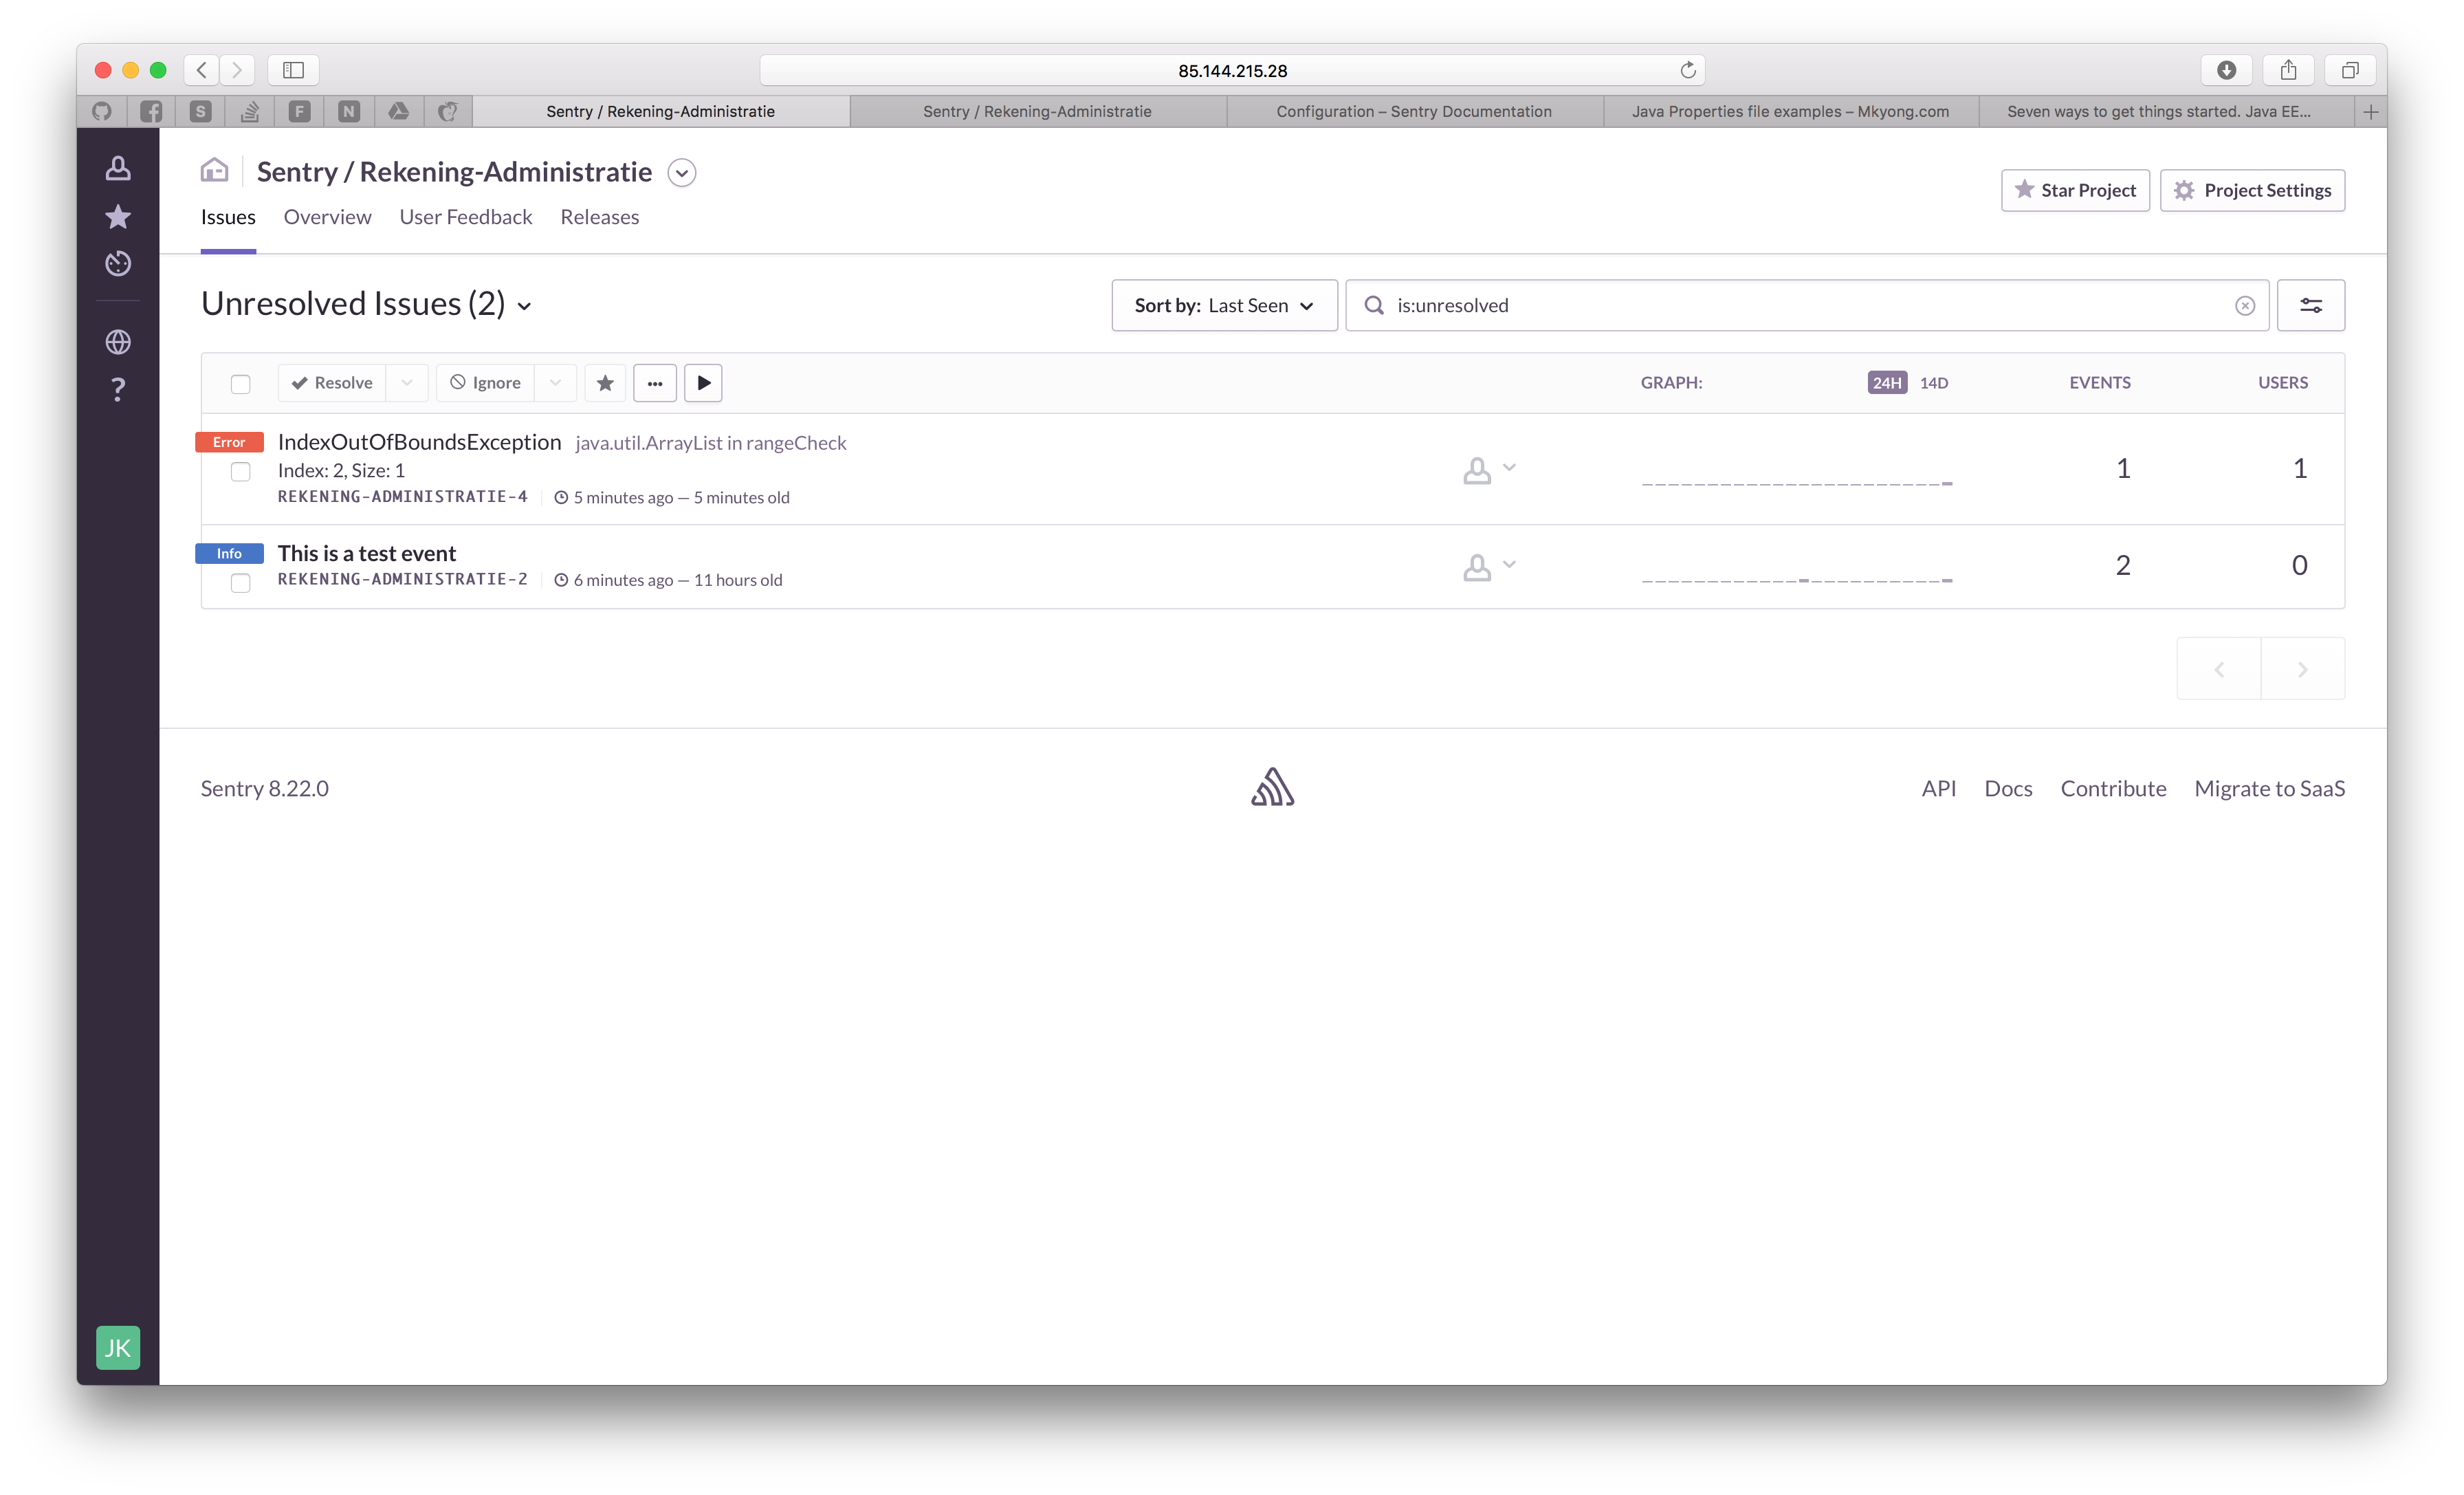
\includegraphics[width=0.95\textwidth]{img/SentryDashboard.png}
	\caption{Sentry dashboard voor Rekening-Administratie project met test exceptions}
	\label{fig:SentryDashboard}
\end{figure}
\newpage
\subsection{Configuratie van Sentry in een Applicatie}
Natuurlijk is het een vereiste om Sentry binnen de verschillende applicaties te configureren. In figuur \ref{fig:SentryApplicatieConfiguratie} is te zien hoe Sentry geinitializeerd wordt binnen een applicatie.
\begin{figure}[H]
	\centering
	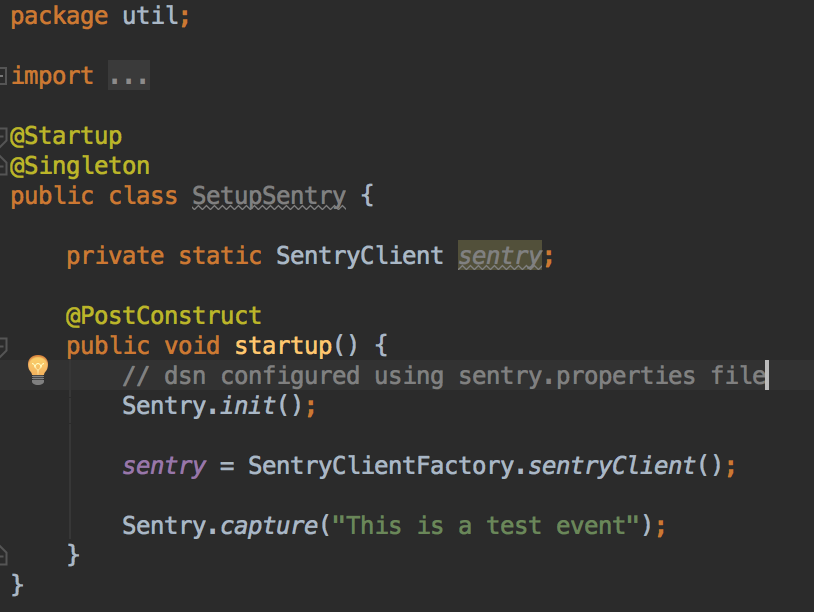
\includegraphics[width=0.50\textwidth]{img/SentryApplicatieConfiguratie.png}
	\caption{Sentry configuratie binnen een applicatie}
	\label{fig:SentryApplicatieConfiguratie}
\end{figure}
Wanneer binnen een applicatie een exception optreedt, kunnen we deze doorsturen aan de hand van onderstaande code.
\begin{lstlisting}
	... 
	} catch (SampleException ex) {
		Sentry.capture(ex);
		// Handel exception af
	}
\end{lstlisting}